\documentclass[../main.tex]{subfiles}

\begin{document}

TO BE COMPLETED

\subsection{Influence of the Wiener CTF correction}
As mentioned in Chapter \ref{chap:implementation}, the approach to tackle the \gls{ctf} of the experimental images consists in correcting them with a Wiener filter. The issue of this approach is that not all frequencies can be recovered due to bad \gls{snr} or zero gain at the \gls{ctf}. Therefore, comparing those frequencies with the reference image may induce an artificial error. The aim of this section is to asses how this phenomenon affects the alignment accuracy.

To do so, several experiments will be carried out. Firstly, simulated images will be aligned with no \gls{ctf} being applied to them (only noise). Obviously, experimental images can not be evaluated without \gls{ctf}, as this is an artefact of the microscope. In any case, this experiment will be useful to observe the accuracy loss that can be attributed to the presence of the \gls{ctf}. 

Moreover, the ground truth alignment parameters of the simulated images are known. Therefore, once the \gls{ctf} has been applied to them, a reconstruction with these images is attempted. This gives an insight on the maximum achievable resolution with the simulated set of images. 

In the second trial, images (both experimental and simulated) will be clustered by their \glspl{ctf}, so that the \gls{ctf} can be assumed to be constant across all images of a given group. Then, each image group can be aligned against a reference set filtered with the representative \gls{ctf} of that group. This approach, similar to the one followed by current refinement packages, will establish the baseline for the alignment accuracy comparison. Lastly, the \gls{ctf} will be corrected with a Wiener filter, and then these images will be aligned against a clean set of reference images. This will give an insight about the alignment quality degradation induced by aligning with Wiener corrected experimental images. 

Earlier, it was stated that most of the alignment information is contained below the resolution of $8\si{\angstrom}$. However, this alignment method targets the initial cycles of the refinement loop, where the reference volume has much less resolution. Therefore, these experiments will be carried out with a resolution limit of $15\si{\angstrom}$, so that the algorithm is evaluated on its operational range. At this resolution, typical \glspl{ctf} have one or two zero crossings. To ensure that the alignment errors can be attributed to the usage of the Wiener filter, no vector compression techniques will be used in these tests.

The tests have proved that using a Wiener filter to correct the \gls{ctf} of the images does not pose a significant penalty respect to applying the \gls{ctf} to the reference images. As shown in Figure \ref{fig:5:ctf_angle_accuracy}, the angle assignment error only increases by $1 \si{\percent}$ on average, whilst Figure \ref{fig:5:ctf_shift_accuracy} shows that shift assignment error increases by a factor of $5 \si{\percent}$. 

It can be noted that the angular assignment error for EMPIAR-10028 is considerably higher than the rest. This is because the calumnium bound to the TPRV5 protein exhibits mismatched symmetry. This means that there is a predominant symmetry which is not followed across all the regions of the protein. In this case, the TPRV5 protein has C4 symmetry but the calumnium is bound off-centred, breaking ensemble's symmetry. As a consequence, it is not easy to distinguish between 

\begin{figure}[htbp]
    \centering
    \begin{subfigure}[b]{.8\textwidth}
         \centering
         %\includegraphics[width=\linewidth]{results/ctf/simulated/angle error}
         \caption{Simulated images}
    \end{subfigure}\\
    \vspace{2em}
    \begin{subfigure}[b]{.8\textwidth}
         \centering
         \includegraphics[width=\linewidth]{results/ctf/experimental/angle error}
         \caption{Experimental images}
    \end{subfigure}
    \caption{Angle accuracy for different compression methods}
    \label{fig:5:ctf_angle_accuracy}
\end{figure}

\begin{figure}[htbp]
    \centering
    \begin{subfigure}[b]{.8\textwidth}
         \centering
         %\includegraphics[width=\linewidth]{results/ctf/simulated/shift error}
         \caption{Simulated images}
    \end{subfigure}\\
    \vspace{2em}
    \begin{subfigure}[b]{.8\textwidth}
         \centering
         \includegraphics[width=\linewidth]{results/ctf/experimental/shift error}
         \caption{Experimental images}
    \end{subfigure}
    \caption{Shift accuracy for different compression methods}
    \label{fig:5:ctf_shift_accuracy}
\end{figure}

\begin{figure}[htbp]
    \centering
    \begin{subfigure}[b]{.8\textwidth}
         \centering
         %\includegraphics[width=\linewidth]{results/ctf/simulated/resolution}
         \caption{Simulated images}
    \end{subfigure}\\
    \vspace{2em}
    \begin{subfigure}[b]{.8\textwidth}
         \centering
         \includegraphics[width=\linewidth]{results/ctf/experimental/resolution}
         \caption{Experimental images}
    \end{subfigure}
    \caption{Reconstruction resolution for different compression methods}
    \label{fig:5:ctf_resolution}
\end{figure}

\subsection{Influence of the vector compression}
One of the key innovations of this algorithm is that it performs efficient vector searches using vector compression techniques. The aim of this section is to assess the effectiveness of such compression and evaluate its influence on the quality of the results.

Several compression techniques will be considered in order to select the best compromise between speed and accuracy. Similarly to the previous experiments, the tests will be carried out with a resolution limit of $15 \si{\angstrom}$. For reference, an alignment without any vector compression will also be considered. The raw input vectors have on average around $1300$ components, which require $5200 \si{\byte}$ to be stored in 32 bit floating point format.

The first evaluated compression technique will be a \gls{pca}. As stated in chapter \ref{chap:implementation}, this compression technique reduces the dimensionality though a linear projection in such a way that most of the signal energy is kept. In this case, input vectors will be reduced to $128$ and $64$ components, leading to an approximate compression rate of x10 and x20, respectively. These vectors will have a constant storage cost of $512\si{\byte}$ and $256\si{\byte}$. Additionally the \gls{pca} projection matrix needs to be stored, which has a inappreciable size when a large quantity of vectors is used.

Secondly, the \gls{ivf}-\gls{pq} vector compression technique described in Chapter \ref{chap:implementation} will be tested. In this case, each block of the vector will be quantised into 256 cells, so that a single byte can be used to represent it. The vector will be divided either in 48 or 32 blocks, so that $48\si{\byte}$ or $32\si{\byte}$ are needed to store it. In this case, the compression ratios are in the order of x100.

The Figure \ref{fig:5:vector_size} illustrates the storage costs for each of the vector compression techniques. Compressed vectors have a size that is agnostic of the dataset. However, the size of the raw vector depends on the image size and its sampling rate. Therefore, the plot shows bars for each of the datasets, although only the first bar varies across acquisitions. Note that the vertical axis of the graph is logarithmic, suggesting that there is an order of magnitude of difference between not using any compression, using \gls{pca} compression and using \gls{ivf}-\gls{pq} compression.

\begin{figure}[htbp]
    \centering
    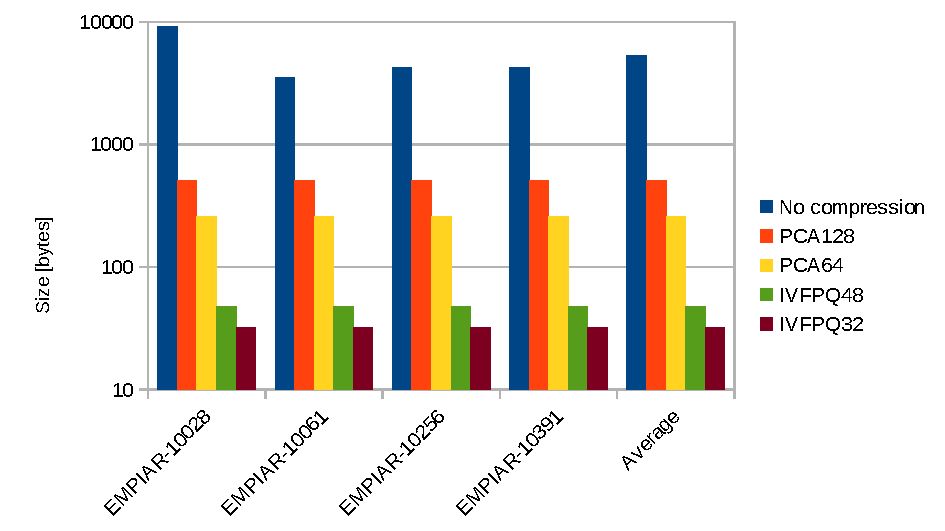
\includegraphics[width=.8\textwidth]{results/compression/vector size}
    \caption{Vector size comparison between vector compression techniques}
    \label{fig:5:vector_size}
\end{figure}


\begin{figure}[htbp]
    \centering
    \begin{subfigure}[b]{.8\textwidth}
         \centering
         \includegraphics[width=\linewidth]{results/compression/simulated/angle error}
         \caption{Simulated images}
    \end{subfigure}\\
    \vspace{2em}
    \begin{subfigure}[b]{.8\textwidth}
         \centering
         \includegraphics[width=\linewidth]{results/compression/experimental/angle error}
         \caption{Experimental images}
    \end{subfigure}
    \caption{Angle accuracy for different vector compression methods}
    \label{fig:5:compression_angle_accuracy}
\end{figure}

\begin{figure}[htbp]
    \centering
    \begin{subfigure}[b]{.8\textwidth}
         \centering
         \includegraphics[width=\linewidth]{results/compression/simulated/shift error}
         \caption{Simulated images}
    \end{subfigure}\\
    \vspace{2em}
    \begin{subfigure}[b]{.8\textwidth}
         \centering
         \includegraphics[width=\linewidth]{results/compression/experimental/shift error}
         \caption{Experimental images}
    \end{subfigure}
    \caption{Shift accuracy for different vector compression methods}
    \label{fig:5:compression_shift_accuracy}
\end{figure}

\begin{figure}[htbp]
    \centering
    \begin{subfigure}[b]{.8\textwidth}
         \centering
         \includegraphics[width=\linewidth]{results/compression/simulated/resolution}
         \caption{Simulated images}
    \end{subfigure}\\
    \vspace{2em}
    \begin{subfigure}[b]{.8\textwidth}
         \centering
         \includegraphics[width=\linewidth]{results/compression/experimental/resolution}
         \caption{Experimental images}
    \end{subfigure}
    \caption{Reconstruction resolution for different vector compression methods}
    \label{fig:5:compression_resolution}
\end{figure}


\subsection{Influence of the cutoff frequency}

\subsection{Combined influence of considered factors}


\end{document}
